% !TeX root = ../main.tex
\chapter{预测}\label{ch6}

第一类应用,例如面部识别、情感分析、对象检测或语音识别,需要从可用信号中预测未知值。

\section{图像去噪}\label{sec6.1}

将深度模型直接应用于图像处理的一个具体应用是利用图像的统计结构中的冗余来从退化中恢复图像。例如,在一张灰度图片中,向日葵的花瓣可以以高置信度进行着色,而几何形状的纹理,例如低光、颗粒状图片上的桌子,可以通过在可能均匀的大区域上进行平均来校正。

\keyterm{去噪自动编码器}是一种模型,它将受损的信号 $\tilde{X}$ 作为输入,并计算出原始信号 $X$ 的估计。对于图像,它是一个可以集成跳跃连接的卷积网络,特别是组合早期获得的相同分辨率的表示 在模型的后期,以及注意层,以方便考虑彼此相距较远的元素。对于图像来说,它是一个卷积网络,可能会集成跳跃连接,尤其是为了组合在模型前期和后期获得的同一分辨率的表示,以及注意力层,以便考虑彼此距离较远的元素。

这样的模型是通过收集大量干净样本及其对应的受损输入来训练的。后者可以在低光或聚焦不足等退化条件下捕获,也可以通过算法生成,例如通过将干净的样本转换为灰度、减小其大小或使用有损压缩方法对其进行激进压缩。

去噪自动编码器的标准训练过程使用所有像素的 MSE 损失之和,在这种情况下,在这种情况下,模型的目标是在给定受损图片的情况下计算出最佳的平均干净图片,即 $E[X \mid \tilde{X}]$。当 $X$ 不完全由 $\tilde{X}$ 确定时,这个量可能是有问题的,在这种情况下,生成信号的某些部分可能是不切实际的、模糊的平均值。

\section{图像分类}\label{sec6.2}

图像\keyterm{分类}是从图像中提取语义的最简单策略,包括在给定输入图像的情况下,从有限的、预定义数量的类别中预测类别。

此任务的标准模型是卷积网络,例如 ResNets(详见 \ref{sec5.2} 节),以及基于注意力的模型,例如 ViT(详见 \ref{sec5.3} 节)。这些模型生成一个 logits 向量,其维度与类别的数量一样多。

训练过程只是最小化交叉熵损失(详见 \ref{sec3.1} 节)。通常,可以通过\keyterm{数据增强}来提高性能,数据增强包括使用手工设计的随机变换修改训练样本,这些变换不会改变图像的语义内容,例如裁剪、缩放、镜像或颜色变化。

\section{对象检测}\label{sec6.3}

图像理解的一个更复杂的任务是\keyterm{对象检测},其目标是在给定输入图像的情况下预测感兴趣对象的类别和位置。

对象位置被形式化为矩形边界框的四个坐标 $(x_1,y_1,x_2,y_2)$,与每个训练图像相关联的真实值是这样的边界框列表,每个边界框都标有其中包含的对象的类别。

解决这一任务的标准方法,例如通过\keyterm{单次检测器}(\keyterm{SSD})\citep{arxiv-1512.02325},是使用卷积神经网络产生一系列大小为 $D_s \times H_s \times W_s$ 的图像表示 $Z_s$,其中 $s = 1, \dots, S$。空间分辨率 $H_s \times W_s$ 逐渐减小,直至 $s = S$ 时缩小为 $1 \times 1$(见图 \ref{fig6.1})。这些张量中的每一个都完全覆盖输入图像,因此 $h,w$ 索引对应于将图像划分为规则正方形,当 $s$ 增加时,规则正方形会变得更加粗糙。

\begin{figure}
    \centering
    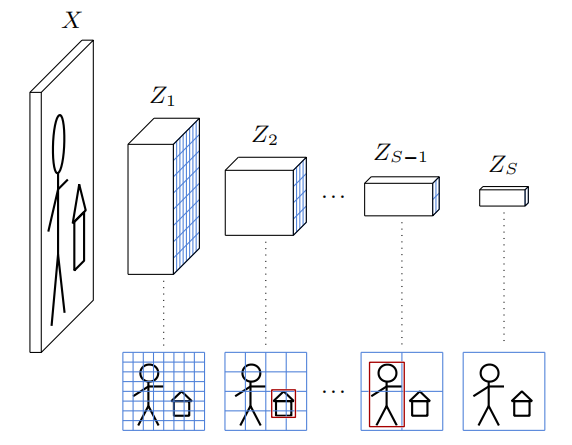
\includegraphics[width=0.9\textwidth]{fig/fig6.1.png}
    \caption[卷积物体检测器]{卷积对象检测器处理输入图像以生成一系列分辨率递减的表示。它在每个尺度 $s$ 上为每个 $h,w$ 计算预定义数量的边界框,这些边界框的中心位于与该单元相对应的图像区域中,并且其大小适合其接受范围。每个预测均采用估计值 ($\hat{x}_1, \hat{x}_2, \hat{y}_1, \hat{y}_2$) 的形式,由上面的红色框表示,以及 $C + 1$ 个 Logits 组成的向量,表示 $C$ 个感兴趣的类别和一个附加的``无对象''类别。}
    \label{fig6.1}
\end{figure}

如 \ref{sec4.2} 节和图 \ref{fig4.4} 所示,由于\keyterm{卷积层}的连续性,特征向量 $(Z_s[0,h,w],\dots,Z_s[D_s-1,h,w])$ 是图像区域的描述符,称为其\keyterm{感受野},它比这个正方形大,但以它为中心。这导致任何边界框 $(x_1,x_2,y_1,y_2)$ 与 $s,h,w$ 的明确匹配,分别由 $\text{max}(x_2-x_1,y_2-y_1), \frac{y_1+y_2}{2}, \frac{x_1+x_2}{2}$ 确定。

检测是通过添加 $S$ 个卷积层来实现的,每个卷积层处理一个 $Z_s$ 并为每个张量索引 $h,w$ 计算边界框的坐标和相关的 logits 值。如果有 $C$ 个对象类别,就会有 $C + 1$ 个 logits 值,额外的一个表示``无对象''。因此,每个附加卷积层都有 $4 + C + 1$ 个输出通道。SSD 算法特别为每个 $s,h,w$ 生成多个边界框,每个边界框专用于硬编码的长宽比范围。

由于使用边界框进行标注需要人工缓慢地干预,因此创建用于对象检测的训练集成本较高。为了缓解这个问题,标准方法是从一个在大型分类数据集上\keyterm{预训练}过的卷积模型开始,比如原始 SSD 使用 VGG-16,然后用额外的卷积层替换其最后的全连接层。令人惊讶的是,尽管对象检测任务涉及到几何量的回归,但仅为分类任务训练的模型所学习到的特征表示却可以重用于对象检测。

在训练过程中,每个真实边界框都与其 $s,h,w$ 相关联,并引入一个损失项,该损失项由 logits 的交叉熵损失和边界框坐标的回归损失(例如 MSE)组成。其他没有边界框匹配的 $s,h,w$ 会引发仅交叉熵惩罚来预测``无对象''类。

\begin{figure}
    \centering
    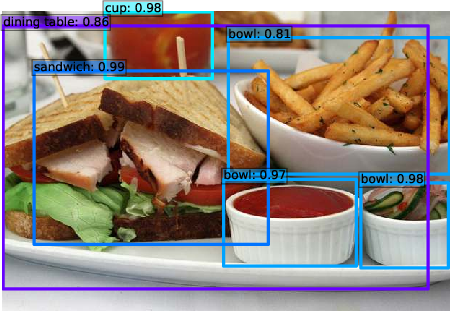
\includegraphics[width=0.8\textwidth]{fig/fig6.2-1.png}
    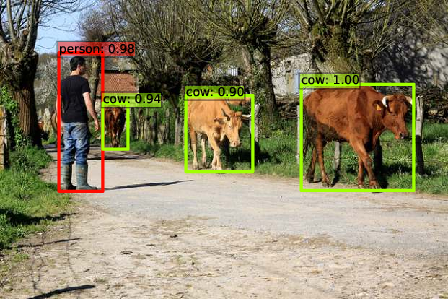
\includegraphics[width=0.8\textwidth]{fig/fig6.2-2.png}
    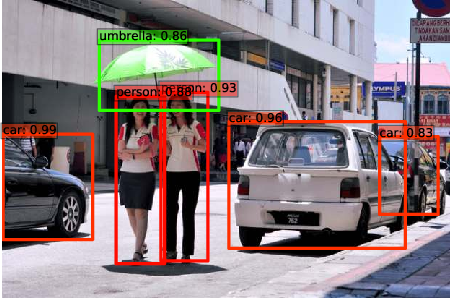
\includegraphics[width=0.8\textwidth]{fig/fig6.2-3.png}
    \caption[使用 SSD 进行物体检测]{使用单次检测器进行物体检测的示例 \citep{arxiv-1512.02325}}
    \label{fig6.2}
\end{figure}

\section{语义分割}\label{sec6.4}

图像理解中最精细的预测任务是\keyterm{语义分割},它涉及预测每个像素所属物体的类别。这可以通过一个标准的卷积神经网络来实现,该网络输出一个卷积图,其中包含与类别数量相同的通道,为每个像素携带估计的 logits 值。

例如,一个标准的残差网络可以生成与其输入相同分辨率的密集输出,就像物体检测一样,这项任务需要在多个尺度上进行操作。这是必要的,以便任何对象或信息丰富的子部分,无论其大小如何,都可以通过单个张量位置的特征表示在模型中的某个位置捕获。因此,这项任务的标准架构会通过一系列\keyterm{卷积层}来缩小图像尺寸,以增大激活的感受野,然后通过一系列\keyterm{转置卷积层}或其他上采样方法(如双线性插值)来重新放大图像,以便进行高分辨率的预测。

\begin{figure}
    \centering
    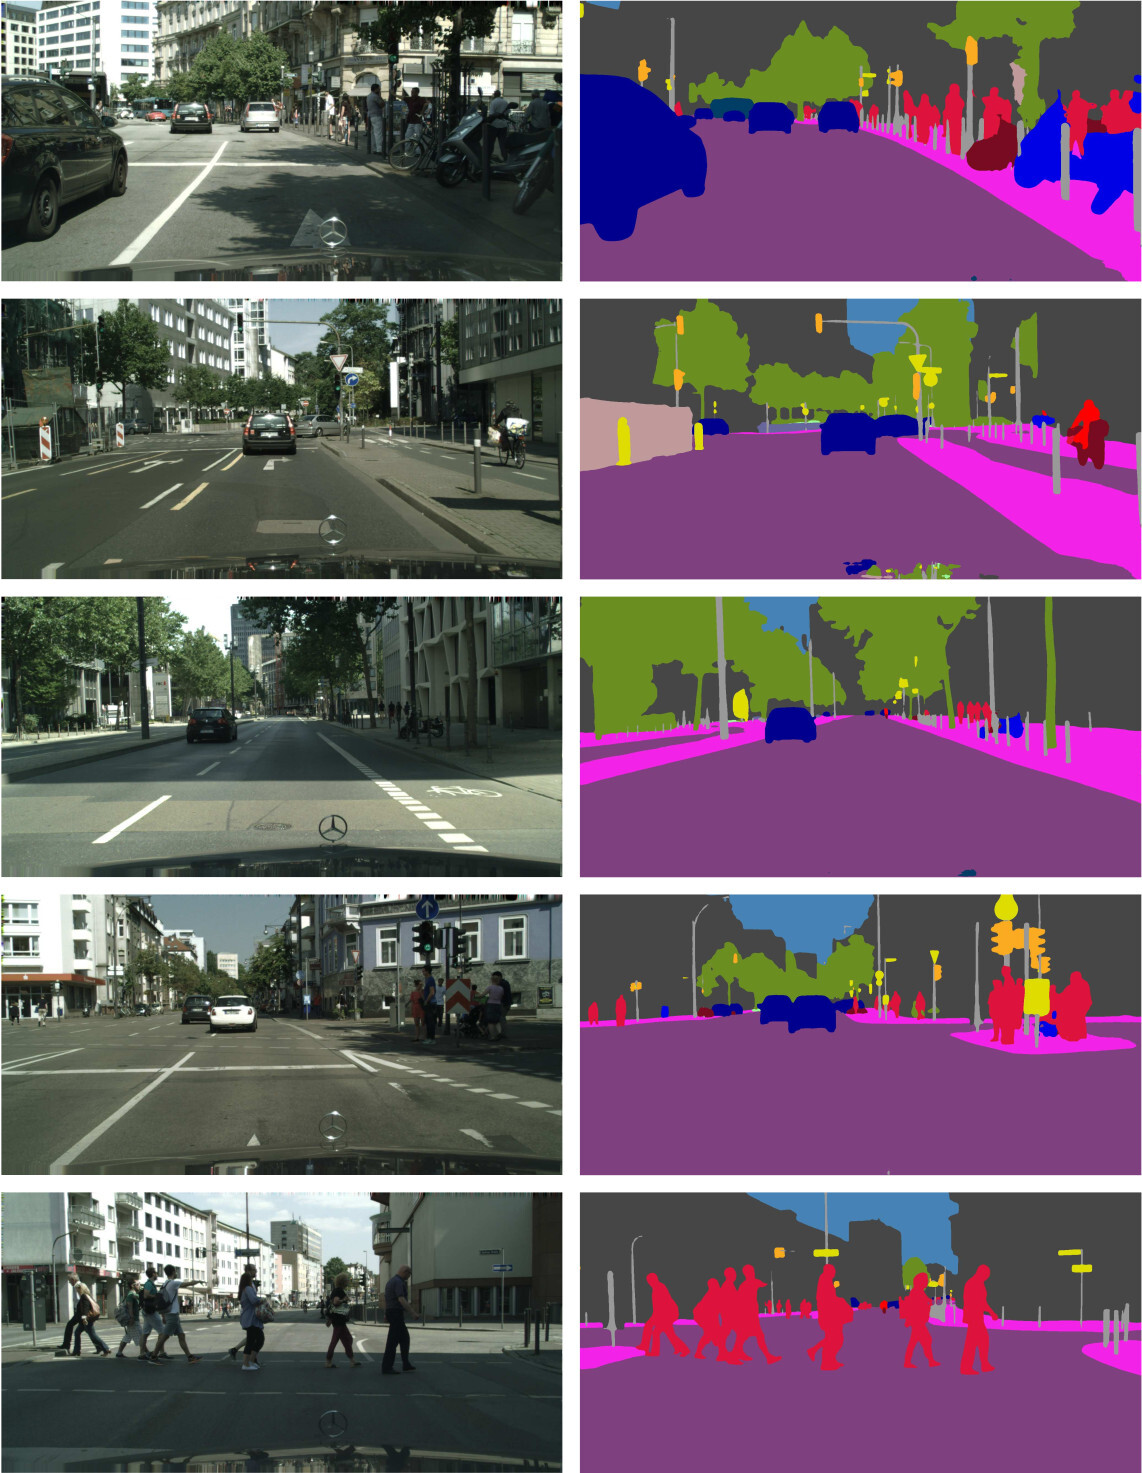
\includegraphics[width=0.9\textwidth]{fig/fig6.3.png}
    \caption[用 PSP 进行语义分割]{金字塔场景分析网络的语义分割结果 \citep{arxiv-1612.01105}}
    \label{fig6.3}
\end{figure}

然而,严格的下采样-上采样架构不允许在进行最终预测时进行细粒度的操作,因为所有的信号在某个时刻都通过了低分辨率的表示。应用这种下采样-上采样的模型通过从缩小之前的特定分辨率的层到放大之后的相同分辨率的层的\keyterm{跳跃连接}来连续缓解这些问题 \citep{arxiv-1411.4038, arxiv-1505.04597}。并行执行此操作的模型,在卷积主干之后,在进行最终的每像素预测之前,在上采样后连接所得的多尺度表示 \citep{arxiv-1612.01105}。

训练是通过对所有像素求和的标准交叉熵来实现的。与对象检测一样,为了弥补分割真值数据有限的问题,训练可以从在大规模图像分类数据集上\keyterm{预训练的网络}开始。

\section{语音识别}\label{sec6.5}

\keyterm{语音识别}包括将声音样本转换为单词序列。历史上有很多解决这个问题的方法,但 Radford \cite{arxiv-2212.04356} 最近提出的一种概念上简单的方法包括将其视为序列到序列的翻译,然后使用标准的基于注意力的 \keyterm{Transformer} 来解决它,如 \ref{sec5.3} 节中所述。

他们的模型首先将声音信号转换为频谱图,该频谱图是一个一维序列 $T \times D$,在每个时间步编码 $D$ 个频带中的能量向量。 关联的文本使用 \keyterm{BPE 分词器}进行编码(参见 \ref{sec3.2} 节)。

频谱图通过几个一维\keyterm{卷积层}进行处理,并将得到的表示输入到 Transformer 的编码器中。解码器直接生成离散的标记序列,其对应于训练期间考虑的可能任务之一。考虑多个目标:英语或非英语文本的转录、从任何语言到英语的翻译、或非语音序列的检测,例如背景音乐或环境噪音。

这种方法可以利用极其庞大的数据集,将多种类型的声源与不同的基本事实相结合。

值得注意的是,尽管这种方法的最终目标是在给定输入信号的情况下产生尽可能确定的翻译,但它形式上是对声音样本条件下的文本分布进行采样,因此这是一个合成过程。事实上,解码器与 \ref{sec7.1} 节的生成模型极其相似。

\section{文本图像表示}\label{sec6.6}

一种强大的图像理解方法包括学习一致的图像和文本表示,这样一来,无论是一幅图像还是其文本描述,都会被映射到同一个特征向量上。

\cite{arxiv-2103.00020} 提出的\keyterm{对比语言-图像预训练}(\keyterm{CLIP})结合了图像编码器 $f$,即 ViT 和文本编码器 $g$,即 GPT。两者均可参见 \ref{sec5.3} 节。

为了将 GPT 重新用作文本编码器,而不是标准的自回归模型,他们向输入序列添加了``句末''标记,并使用最后一层中该标记的表示作为嵌入。 其尺寸在 $512$ 到 $1024$ 之间,具体取决于配置。

这两个模型使用从 Internet 收集的 4 亿张图像文本对 $(i_k,t_k)$ 从头开始训练。训练过程遵循标准的小批量随机梯度下降法,但依赖于\keyterm{对比损失}。对于小批量中的 $N$ 对图像和文本,都会计算出相应的嵌入向量,并计算每对图像与文本嵌入向量之间的余弦相似度,还会计算跨对之间的相似度,从而得到一个 $N \times N$ 矩阵的相似度得分:
\[l_{m,n} = f(i_m) \cdot g(t_n), m = 1,\dots,N, n = 1,\dots,N\]
模型使用交叉熵进行训练,$\forall n$ 值 $l_{1,n},\dots,l_{N,n}$ 被解释为预测 $n$ 的 logit 分数,$l_{n,1},\dots,l_{n,N}$ 与之类似。这意味着 $\forall n,m, \text{s.t.} n \ne m$ 时,相似度 $l_{n,n}$ 严格大于 $l_{n,m}$ 和 $l_{m,n}$。

训练完成后,该模型可用于\keyterm{零样本预测},即在没有训练样例的情况下对信号进行分类。方法是定义一系列带有文本描述的候选类别,并计算图像嵌入向量与这些描述中每一个嵌入向量的相似度(见图 \ref{fig6.4})。

\begin{figure}
    \centering
    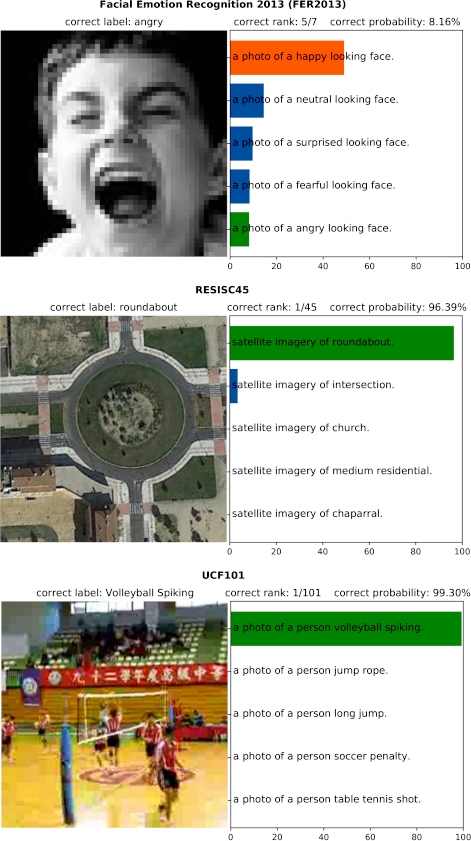
\includegraphics[width=0.9\textwidth]{fig/fig6.4.png}
    \caption[CLIP 零样本预测]{CLIP 文本图像嵌入 \citep{arxiv-2103.00020} 允许通过预测哪类描述嵌入与图像嵌入最一致来进行零样本预测。}
    \label{fig6.4}
\end{figure}

此外,由于文本描述通常更为详细,这样的模型需要捕捉图像更丰富的表示,并且识别出超出常规分类所需的线索。这意味着在一些具有挑战性的数据集上,例如专门设计用来降低或消除标准预测器依赖的线索的数据集 ImageNet Adversarial \citep{arxiv-1907.07174},该模型展现出了出色的性能。

\section{强化学习}\label{sec6.7}

许多问题,例如策略游戏或机器人控制,都可以用离散时间状态过程 $S_t$ 和通过选择行动 $A_t$ 来调节的奖励过程 $R_t$ 来形式化。如果 $S_t$ 具有\keyterm{马尔可夫性},意味着它本身携带的关于未来的信息与直到那一刻为止的所有过去状态一样多,这样的对象就是一个\keyterm{马尔可夫决策过程}(\keyterm{MDP})。

给定 MDP,目标通常是找到一个\keyterm{策略} $\pi$,使得 $A_t = \pi(S_t)$ 能够最大化\keyterm{回报}的期望,这个回报是一种累积折扣奖励:

\[\mathbb{E}\Bigg[\sum_{t \ge 0}\gamma^tR_t\Bigg]\]

折扣因子满足 $0 < \gamma < 1$。

这是\keyterm{强化学习}(\keyterm{RL})的标准设置,可以通过引入最优状态-动作价值函数 $Q(s,a)$ 来解决这一问题,该函数是我们在状态 $s$ 执行动作 $a$ 并遵循最优策略的期望回报。它提供了一种计算最优策略的方法,即 $\pi(s) = \argmax_aQ(s,a)$,并且由于马尔可夫假设,它验证了\keyterm{贝尔曼方程}:
\begin{equation}
    \begin{aligned}
    Q&(s,a) = \\
    &\mathbb{E}\Big[R_t +\gamma \underset{a'} \max Q(S_{t+1},a') \mid S_t = s,A_t = a\Big] \label{eq6.1}
    \end{aligned}
\end{equation}
我们可以据此设计一个程序来训练参数模型 $Q(\cdot, \cdot ;w)$。

为了应用这个框架来玩经典的 Atari 视频游戏,\cite{nature14236} 使用时间 $t$ 帧和之前的三个帧的串联作为 $S_t$,以便马尔可夫假设成立,并使用一个被称为\keyterm{深度 Q 网络}(\keyterm{DQN})的模型作为 $Q$,由两个卷积层和一个全连接层组成,每个动作一个输出值,遵循 LeNet 的经典结构(参见 \ref{sec5.2} 节)。

训练是通过交替进行游戏和记录游戏场景来实现的,并构建小批量的元组 $(s_n,a_n,r_n,s'_n)\sim(S_t,A_t,R_t,S_{t+1})$,这些元组跨存储的游戏场景和时间步选取,并通过一次随机梯度下降(SGD)迭代来最小化
\begin{equation}
    \mathcal{L}(w)= \frac{1}{N}\sum_{n=1}^{N}\big(Q(s_n,a_n;w)-y_n\big)^2 \label{eq6.2}
\end{equation}
其中,如果这个元组是游戏场景的结尾,则 $y_n = r_n$;否则,$y_n = r_n + \gamma \max_aQ(s'_n,a; \bar{w})$。

这里 $\bar{w}$ 是 $w$ 的常量副本,即梯度不会通过它传播到 $w$。这是必要的,因为公式 \ref{eq6.1} 中的目标值是 $y_n$ 的期望,而公式 \ref{eq6.2} 中使用的是 $y_n$ 本身。固定 $y_n$ 中的 $w$ 可以更好地近似所需的梯度。

一个关键问题是用于收集游戏场景的策略。\cite{nature14236} 简单地使用了 $\varepsilon$-贪婪策略,该策略包括以 $\varepsilon$ 的概率完全随机地采取一个行动,其余情况下采取最优行动 $\argmax_aQ(s,a)$。引入一些随机性是必要的,有助于促进探索。

训练是用一千万帧完成的,相当于不到八天的游戏时间。经过训练的网络可以计算状态值的准确估计(见图 \ref{fig6.5}),并在用于实验验证的 49 款游戏中的大多数上达到了人类的表现水平。

\begin{figure}
    \centering
    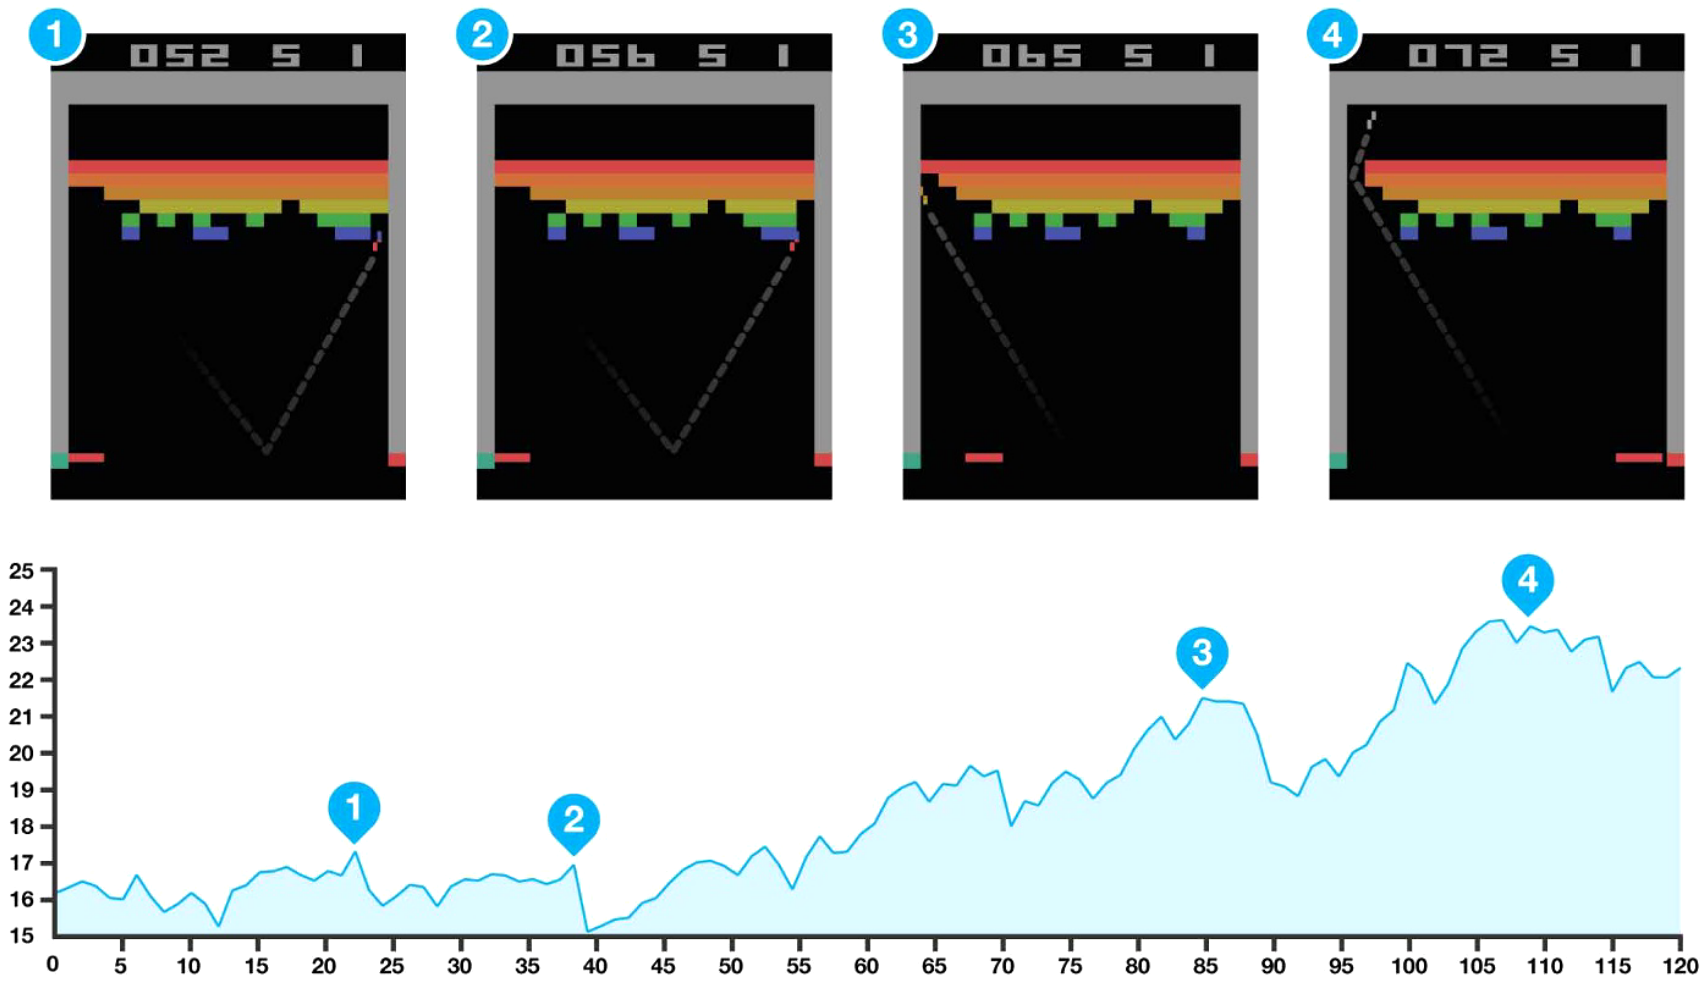
\includegraphics[width=0.9\textwidth]{fig/fig6.5.png}
    \caption[DQN 状态值演化]{该图显示了打砖块游戏期间状态值 $V(S_t)=\max_aQ(S_t,a)$ 的演变。时间点 (1) 和 (2) 处的尖峰对应于清除砖块,在时间点 (3) 处,砖块即将突破顶线,在 (4) 处确实突破了顶线,这确保了未来的高奖励 \citep{nature14236}。}
    \label{fig6.5}
\end{figure}